% \documentclass[paper=a4, fontsize=11pt]{scrartcl} % A4 paper and 11pt font size
\documentclass[a4paper,11pt]{book}
%\usepackage[T1]{fontenc} % Use 8-bit encoding that has 256 glyphs
\usepackage[utf8]{inputenc}
\usepackage{fourier} % Use the Adobe Utopia font for the document - comment this line to return to the LaTeX default
\usepackage{listings} % para insertar código con formato similar al editor
\usepackage[spanish, es-tabla]{babel} % Selecciona el español para palabras introducidas automáticamente, p.ej. "septiembre" en la fecha y especifica que se use la palabra Tabla en vez de Cuadro
\usepackage{url} % ,href} %para incluir URLs e hipervínculos dentro del texto (aunque hay que instalar href)
\usepackage{graphics,graphicx, float} %para incluir imágenes y colocarlas
\usepackage[gen]{eurosym} %para incluir el símbolo del euro
\usepackage{cite} %para incluir citas del archivo <nombre>.bib
\usepackage{enumerate}
\usepackage{hyperref}
\usepackage{tabularx}
\usepackage{booktabs}
\usepackage{afterpage}
\usepackage{longtable}
\usepackage[stable]{footmisc}
\usepackage[table,xcdraw]{xcolor}



% ********************************************************************
% Re-usable information
% ********************************************************************
\newcommand{\myTitle}{Técnicas de Deep Learning para el diagnóstico del Alzheimer\xspace}
\newcommand{\myDegree}{Grado en Ingeniería Informática\xspace}
\newcommand{\myName}{Raquel Molina Reche\xspace}
\newcommand{\myProf}{Rosa María Rodriguez Sánchez\xspace}
\newcommand{\myFaculty}{Escuela Técnica Superior de Ingenierías Informática y de
Telecomunicación\xspace}
\newcommand{\myFacultyShort}{E.T.S. de Ingenierías Informática y de
Telecomunicación\xspace}
\newcommand{\myDepartment}{Departamento de Ciencias de la Computación e Inteligencia Artificial\xspace}
\newcommand{\myUni}{\protect{Universidad de Granada}\xspace}
\newcommand{\myLocation}{Granada\xspace}
\newcommand{\myTime}{\today\xspace}
\newcommand{\myVersion}{Version 0.1\xspace}


\hypersetup{
    colorlinks=true,	% false: boxed links; true: colored links
    linkcolor=black,	% color of internal links
    urlcolor=cyan		% color of external links
}


\renewcommand{\familydefault}{\sfdefault}
\usepackage{fancyhdr} % Custom headers and footers
\pagestyle{fancyplain} % Makes all pages in the document conform to the custom headers and footers
\fancyhead[L]{} % Empty left header
\fancyhead[C]{} % Empty center header
%\fancyhead[R]{Me Llamo Así} % My name
\fancyfoot[L]{} % Empty left footer
%\fancyfoot[C]{} % Empty center footer
\fancyhf{}
\fancyhead[LO]{\leftmark}
\fancyhead[RE]{\rightmark}
\fancyhead[RO,LE]{\textbf{\thepage}}
\fancyfoot[C]{\thepage} % Page numbering for center footer
%\renewcommand{\headrulewidth}{0pt} % Remove header underlines
\renewcommand{\footrulewidth}{0pt} % Remove footer underlines
\setlength{\headheight}{13.6pt} % Customize the height of the header
\renewcommand{\chaptermark}[1]{\markboth{\textbf{#1}}{}}
\renewcommand{\sectionmark}[1]{\markright{\textbf{\thesection. #1}}}

\usepackage{titlesec, blindtext, color}
\definecolor{gray75}{gray}{0.75}
\newcommand{\hsp}{\hspace{20pt}}
\titleformat{\chapter}[hang]{\Huge\bfseries}{\thechapter\hsp\textcolor{gray75}{|}\hsp}{0pt}{\Huge\bfseries}
\setcounter{secnumdepth}{4}
\usepackage[Lenny]{fncychap}

\setlength{\headheight}{1.5\headheight}

\newcommand{\HRule}{\rule{\linewidth}{0.5mm}}
\newcommand{\bigrule}{\titlerule[0.5mm]}


%Definimos los tipos teorema, ejemplo y definición podremos usar estos tipos
%simplemente poniendo \begin{teorema} \end{teorema} ...
\newtheorem{teorema}{Teorema}[chapter]
\newtheorem{ejemplo}{Ejemplo}[chapter]
\newtheorem{definicion}{Definición}[chapter]

\definecolor{gray97}{gray}{.97}
\definecolor{gray75}{gray}{.75}
\definecolor{gray45}{gray}{.45}
\definecolor{gray30}{gray}{.94}

\lstset{ frame=Ltb,
    framerule=0.5pt,
    aboveskip=0.5cm,
    framextopmargin=3pt,
    framexbottommargin=3pt,
    framexleftmargin=0.1cm,
    framesep=0pt,
    rulesep=.4pt,
    backgroundcolor=\color{gray97},
    rulesepcolor=\color{black},
%
    stringstyle=\ttfamily,
    showstringspaces = false,
    basicstyle=\scriptsize\ttfamily,
    commentstyle=\color{gray45},
    keywordstyle=\bfseries,
%
    numbers=left,
    numbersep=6pt,
    numberstyle=\tiny,
    numberfirstline = false,
    breaklines=true,
}

% minimizar fragmentado de listados
\lstnewenvironment{listing}[1][]
{\lstset{#1}\pagebreak[0]}{\pagebreak[0]}

\lstdefinestyle{CodigoC}
{
    basicstyle=\scriptsize,
    frame=single,
    language=C,
    numbers=left
}
\lstdefinestyle{CodigoC++}
{
    basicstyle=\small,
    frame=single,
    backgroundcolor=\color{gray30},
    language=C++,
    numbers=left
}


\lstdefinestyle{Consola}
{basicstyle=\scriptsize\bf\ttfamily,
    backgroundcolor=\color{gray30},
    frame=single,
    numbers=none
}

%Para conseguir que en las páginas en blanco no ponga cabecerass
\makeatletter
\def\clearpage{%
    \ifvmode
    \ifnum \@dbltopnum =\m@ne
    \ifdim \pagetotal <\topskip
    \hbox{}
    \fi
    \fi
    \fi
    \newpage
    \thispagestyle{empty}
    \write\m@ne{}
    \vbox{}
    \penalty -\@Mi
}
\makeatother



\begin{document}

    % Plantilla portada UGR
    \begin{titlepage}


\newlength{\centeroffset}
\setlength{\centeroffset}{-0.5\oddsidemargin}
\addtolength{\centeroffset}{0.5\evensidemargin}
\thispagestyle{empty}

\noindent\hspace*{\centeroffset}\begin{minipage}{\textwidth}

\centering

\includegraphics[width=0.9\textwidth]{logos/logo_ugr.jpg}\\[1.4cm]

\textsc{ \Large TRABAJO FIN DE GRADO\\[0.2cm]}
\textsc{ GRADO EN INGENIERÍA INFORMÁTICA}\\[1cm]
% Upper part of the page
% 
% Title
{\Huge\bfseries Técnicas de Deep Learning para el diagnóstico del Alzheimer\\}
\noindent\rule[-1ex]{\textwidth}{3pt}\\[3.5ex]
%{\large\bfseries Subtitulo del Proyecto}
\end{minipage}


\vspace{2.5cm}

\noindent\hspace*{\centeroffset}\begin{minipage}{\textwidth}
\thispagestyle{empty}
\centering

\textbf{Autor}\\ {Raquel Molina Reche}\\[2.5ex]
\textbf{Director}\\ {Rosa María Rodriguez Sánchez}\\[2cm]

\includegraphics[width=0.3\textwidth]{logos/etsiit_logo.png}\\[0.1cm]
\textsc{Escuela Técnica Superior de Ingenierías Informática y de Telecomunicación}\\
\textsc{---}\\
Granada, Junio de 2022


\end{minipage}
\end{titlepage}




    % Plantilla prefacio UGR
    \thispagestyle{empty}

\begin{center}
{\large\bfseries \myTitle}\\
\end{center}
\begin{center}
       \myName\\
\end{center}

\vspace{0.7cm}
\noindent{\textbf{Palabras clave}: palabra\_clave1, palabra\_clave2, palabra\_clave3, ......}\\

\vspace{0.7cm}
\noindent{\textbf{Resumen}}\\

Poner aquí el resumen.
\cleardoublepage
\thispagestyle{empty}


\begin{center}
{\large\bfseries \myTitleEn}\\
\end{center}
\begin{center}
       \myName\\
\end{center}

\vspace{0.7cm}
\noindent{\textbf{Keywords}: Keyword1, Keyword2, Keyword3, ....}\\

\vspace{0.7cm}
\noindent{\textbf{Abstract}}\\

Write here the abstract in English.

%\cleardoublepage
%\thispagestyle{empty}
%
%\noindent\rule[-1ex]{\textwidth}{2pt}\\[4.5ex]
%
%Yo, \textbf{Raquel Molina Reche}, alumna de la titulación Ingeniería Informática de la \textbf{Escuela Técnica Superior
%de Ingenierías Informática y de Telecomunicación de la Universidad de Granada}, con DNI 49627634M, autorizo la
%ubicación de la siguiente copia de mi Trabajo Fin de Grado en la biblioteca del centro para que pueda ser
%consultada por las personas que lo deseen.
%
%\vspace{6cm}
%
%\noindent Fdo: Raquel Molina Reche
%
%\vspace{2cm}
%
%\begin{flushright}
%Granada a X de mes de 201 .
%\end{flushright}


\cleardoublepage
\thispagestyle{empty}

\noindent\rule[-1ex]{\textwidth}{2pt}\\[4.5ex]

Dª. \textbf{\myProf}, Profesora del \myDepartment de la \myUni.

\vspace{0.5cm}

\textbf{Informa:}

\vspace{0.5cm}

Que el presente trabajo, titulado \textit{\textbf{\myTitle}},
ha sido realizado bajo su supervisión por \textbf{\myName}, y autorizo la defensa de dicho trabajo ante el tribunal
que corresponda.

\vspace{0.5cm}

Y para que conste, expido y firmo el presente informe en \myLocation a \myTime.

\vspace{1cm}

\textbf{La directora:}

\vspace{5cm}

\noindent \textbf{\myProf}

\chapter*{Agradecimientos}
\thispagestyle{empty}

       \vspace{1cm}


Poner aquí agradecimientos...



    %\frontmatter
    %\tableofcontents
    %\listoffigures
    %\listoftables
    %
    %\mainmatter
    %\setlength{\parskip}{5pt}

    %\chapter{Introducción}\label{ch:introduccion}

Este proyecto está publicado bajo la licencia GNU General Public License v3~\cite{gplv3}.
Se puede acceder a través de GitHub en este \href{https://github.com/raquelmolinare/TFG}{enlace}.


\section{Motivación y contexto}\label{sec:motivacion-y-contexto}
A día de hoy, gracias a los avances en ciencias de la computación, la inteligencia artificial (en adelante \Gls{IA}) se está
convirtiendo en una parte fundamental de la atención médica actual.
Algoritmos y aplicaciones impulsadas por IA se usan en el día a día para ayudar a los profesionales en entornos clínicos
y en el ámbito de la investigación.

Según la Confederación Española de Alzheimer (CEAFA)~\cite{ceafa} la \textbf{Enfermedad del Alzheimer} (en adelante \Gls{EA})
es una enfermedad neurodegenerativa que afecta a aproximadamente 1.200.000 personas en España y a más de 50 millones de
personas en el mundo según un artículo de la Universitat Oberta de Catalunya (UOC)~\cite{uoc}.
Es una enfermedad progresiva, o lo que es lo mismo, que empeora con el tiempo y para la que no existe una cura, solo
la posibilidad de aplicar tratamientos que ralenticen su avance.
Para que estos tratamientos no resulten perjudiciales para la salud del paciente deben realizarse en las primeras etapas
de la enfermedad.
Por ello un diagnóstico temprano puede ser determinante para el paciente, pero, en la mayoría de casos, detectar esta
enfermedad en las primeras fases de la misma es una tarea muy compleja.

Investigaciones previas han concluido que las primeras lesiones cerebrales pueden aparecer incluso 20 años antes de que
aparezcan los primeros síntomas del Alzheimer~\cite{ceafa}.
De hecho una de las evaluaciones médicas para la detección de la enfermedad se basa en el diagnóstico por imágenes
cerebrales mediante la realización de un examen imagenológico, que puede incluir técnicas como: Imagen por Resonancia
Magnética (en adelante MRI), Tomografía Computarizada o Tomografía por emisión de positrones (en adelante \Gls{PET}).

A día de hoy el aprendizaje profundo o deep learning (en adelante \Gls{DL})  ha levantado mucho interés en el mundo de la
medicina.
El Deep learning es un subconjunto del machine learning (en adelante \Gls{ML}) en IA, que simula el comportamiento del cerebro
humano en el procesamiento de datos y el reconocimiento de patrones para resolver problemas complejos de toma de
decisiones.

Es por esto que el uso de DL puede ayudar a un diagnóstico temprano, ya que estos sistemas pueden ser utilizados para la
detección de anomalías en imágenes médicas donde destaca la rapidez de la detección, sirviendo como herramienta de
prevención y seguimiento de la enfermedad.

También cabe destacar que la enfermedad del Alzheimer presenta diferentes fases y la velocidad a la que avanza la
enfermedad por las diferentes fases varía, por lo que es más difícil realizar predicciones a largo plazo.
Se usan escalas con distinto número de fases:
\begin{itemize}
    \item \textbf{La escala de deterioro global (GDS)}~\cite{gds} se divide en siete fases que dependen del valor del
    deterioro cognitivo y más común utilizarla para escalar la demencia senil.
    Sus fases son: ausencia de alteración cognitiva, disminución cognitiva muy leve, defecto cognitivo leve, defecto
    cognitivo moderado, defecto cognitivo moderado-grave, defecto cognitivo grave y defecto cognitivo muy grave.
    \item \textbf{La escala de clasificación de la demencia clínica (CDR)}~\cite{cdr} se divide en cinco fases, es la más
    utilizada en el área de investigación y evalúa diferentes parámetros como la memoria, la orientación, la resolución
    de problemas, el juicio, etc.
    Sus fases son: Cognitivamente sano (CDR 0), demencia cuestionable (CDR 0.5), demencia leve (CDR 1), demencia
    moderada (CDR 2) y demencia grave (CDR 3).
    \item \textbf{La escala de clasificación común}~\cite{alz-org-etapas} solo tiene en cuenta tres fases, es la más
    usada en la comunicación médico-familia, ya que es la más sencilla de comprender.
    Las fases que tiene en cuenta son: Enfermedad de Alzheimer leve (etapa temprana), enfermedad de Alzheimer moderada
    (etapa media) y enfermedad de Alzheimer grave (etapa final).\\
\end{itemize}

A día de hoy, realizar estudios en esta área significa conseguir grandes avances en el mundo de la medicina y del
diagnóstico del Alzheimer, ayudando a mejorar la vida de los pacientes y las familias.
Por lo tanto, la motivación de este trabajo se centra en el estudio del uso de técnicas de Deep Learning para el
diagnóstico del Alzheimer a partir de imágenes cerebrales.




\section{Objetivos}\label{sec:objetivos}
El objetivo general de este proyecto es identificar qué plano cerebral ofrece mejor rendimiento para el diagnóstico del
Alzheimer mediante el uso de técnicas de Deep Learning a partir de Imágenes por Resonancia Magnética y facilitar su uso
en una aplicación real.

Este estudio se puede dividir en los siguientes objetivos específicos:
\begin{itemize}
    \item Conocer los conceptos teóricos del cuadro clínico, fases y diagnóstico de la EA.
    \item Estudiar las herramientas de DL y de procesamiento de imágenes más usadas actualmente para el diagnóstico del
    Alzheimer.
    \item Realizar un análisis y tratamiento de biomarcadores de Imagen por Resonancia Magnética.
    \item Analizar y seleccionar la arquitectura del sistema de DL para la resolución del problema.
    \item Evaluar el rendimiento que ofrecen los distintos planos cerebrales: axial, coronal y sagital al aplicar la
    técnica escogida.
    \item Desarrollar una aplicación web como ejemplo de uso real del sistema de aprendizaje profundo generado para
    facilitar la labor de los profesionales de entornos clínicos en el diagnóstico de la EA.\\
\end{itemize}




\section{Metodología, herramientas y obstáculos}\label{sec:metodologia-herramientas-y-obstaculos}
Una vez definidos los objetivos del problema a resolver, se explica a continuación la metodología y herramientas
implicadas en el desarrollo del proyecto y los posibles problemas que pueden surgir.

\subsection{Metodología}\label{subsec:metodologia}
Para conseguir los objetivos del  proyecto se ha seguido un desarrollo ágil en el que se han marcado 2 enfoques
principales:
\begin{itemize}
    \item El Trabajo de Fin de Grado (en adelante \Gls{TFG}) como proyecto, que engloba la construcción del sistema de DL, y
    en el que el cliente es el usuario lector de este trabajo.
    \item La aplicación web como proyecto con profesionales de entornos clínicos como clientes.\\
\end{itemize}

El desarrollo ágil es una metodología de trabajo cuyo objetivo principal es adaptarse a los cambios o necesidades
temporales de un proyecto y está basada en el desarrollo iterativo e incremental.
Mediante esta metodología se puede dividir el proyecto en tareas agrupadas en pequeñas etapas y que mediante su
finalización van añadiendo valor al producto final.

Los métodos ágiles de desarrollo de software usados a día de hoy se fundamentan en el trabajo en equipo, puesto que este
proyecto no está realizado por un equipo, si no que se elabora por una sola persona, se ha decidido seguir una
metodología de desarrollo ágil personalizada basada en los principios de las metodologías ágiles desarrollo de
software comunes:
\begin{itemize}
    \item Perseguir la satisfacción del cliente.
    En este caso del usuario lector y de profesionales de entornos clínicos.
    \item División del trabajo en fases temporales productivas compuestas por tareas simples.
    \item Medición del progreso.
    \item Adaptación a cambios.\\
\end{itemize}

\subsection{Herramientas}\label{subsec:herramientas}
Las herramientas empleadas para conseguir los objetivos del proyecto mediante la metodología explicada anteriormente se
detallan en esta sección.

Para llevar a cabo la medición del progreso se hace uso \textit{GIT} como sistema de control de versiones y
\textit{GitHub} como forja para alojar el proyecto, no solo por ser una herramienta considerablemente conocida y
utilizada en el día a día sin no también porque nos ofrece un amplio abanico de herramientas para construir software
seguro integradas en la propia plataforma como son los \textit{tableros Kanban} o Integración Continua mediante
\textit{GitHub Actions} entre otros.

Para este trabajo se han creado dos proyectos o \textit{tableros Kanban} en \textit{GitHub}, uno para la medición del
progreso del propio TFG y otro para la aplicación web a desarrollar, tal y como se comenta en el apartado anterior.
También se han definido un conjunto de \textit{milestones} para marcar puntos específicos del proyecto que reúnen diversas
\textit{issues}, las cuales tras completarse marcan la finalización del \textit{milestone} al que pertenecen.


\subsubsection{Milestones}
Los \textit{milestones} en este trabajo han señalado productos mínimos viables, de tal manera que completar todos los
\textit{milestones} da lugar a la finalización del proyecto y además se pretende que conforme se vayan completando
\textit{milestones} se vayan concluyendo los distintos objetivos que engloban este proyecto.
Los \textit{milestones} creados han sido los siguientes:
\begin{itemize}
    \item  \textbf{1. Base e introducción}: Preparación del entorno y sistema de trabajo y abarca la parte inicial de la
    memoria y de investigación del proyecto.
    \item \textbf{2. Análisis y Desarrollo experimental}: Desarrollo de un sistema de aprendizaje profundo a partir de
    Imágenes por Resonancia Magnética capaz de predecir el grado de Alzheimer presente en la imagen.
    Atendiendo a la literatura actual recopilada en el primer milestone.
    \item \textbf{3. Desarrollo de la aplicación web}: Construir una app que facilite el diagnóstico de la EA integrando el
    sistema de aprendizaje profundo implementado.
    \item \textbf{4. Conclusión}: Incluye la conclusión final de todo el proyecto y la finalización de los elementos
    introductorios.\\
\end{itemize}

\subsubsection{Historias de usuario}
Dentro de las \textit{issues} de \textit{GitHub} se ha diferenciado entre Historias de Usuario (en adelante \Gls{HU}) o
tareas.
A parte de diferenciarse en la nomenclatura se ha hecho uso de etiquetas para clasificar las \textit{issues}, las cuales
han sido:

\begin{itemize}
    \item \textit{user story}: para marcar HU.
    \item \textit{task}: para marcar tareas.
    \item \textit{research}: para marcar tareas relacionadas con investigación.
    \item \textit{documentation}: para marcar tareas relacionadas con documentación.
    \item \textit{development}: para marcar tareas relacionadas con desarrollo. \\
\end{itemize}

Las HUs  han marcado los objetivos y expresado las necesidades de los usuarios de nuestro proyecto desde su punto de
vista, dando lugar a las siguientes:
\begin{itemize}
    \item \textbf{Como lector quiero poder conocer la envergadura del proyecto de manera sencilla y ordenada a partir de la
    memoria}: Forma parte del concepto del proyecto como TFG. Como criterio de aceptación la memoria debe ser ordenada,
    clara y concisa de forma que se entienda el trabajo.
    \item \textbf{Como lector quiero conocer qué plano cerebral ofrece mejor rendimiento para el diagnóstico de la Enfermedad de
    Alzheimer mediante técnicas de aprendizaje profundo}: Engloba el desarrollo experimental del sistema de DL para el
    diagnóstico de la EA. Como criterio de aceptación  se debe llegar a una conclusión final sobre el plano que ofrece
    mayor rendimiento.
    \item \textbf{Como profesional de entornos clínicos quiero poder conocer el grado de Enfermedad de Alzheimer en una
    resonancia magnética de manera sencilla}:  Engloba el desarrollo de la aplicación web y se detalla más detenidamente
    en el capítulo~\ref{ch:aplicacion-web-para-el-diagnostico-del-alzheimer-mediante-mri}. \\
\end{itemize}

\begin{figure}[H]
    \centering
    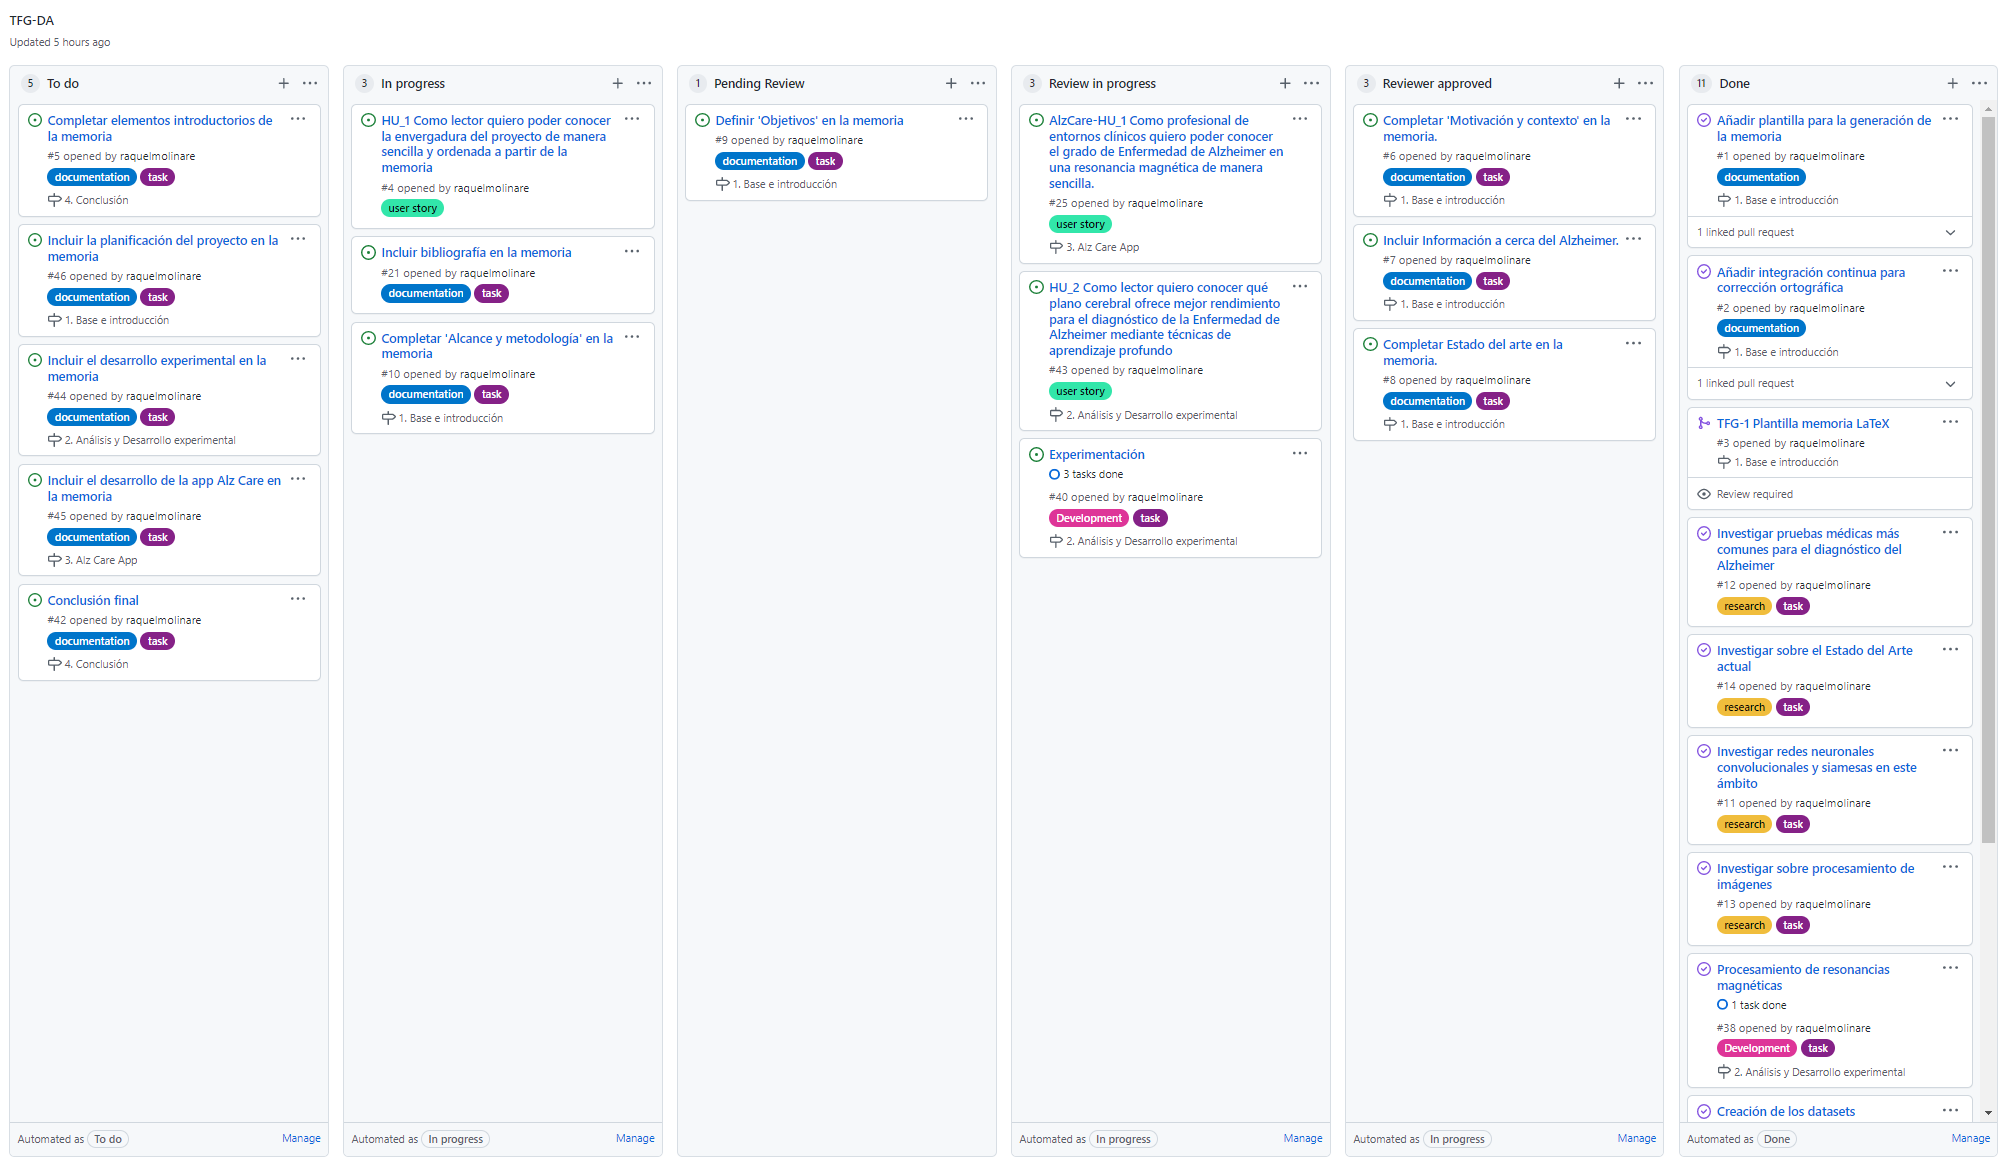
\includegraphics[width=\textwidth]{./imgs/tablero-github}
    \caption{Tablero Kanban del TFG desde GitHub}
    \label{fig:tablero-kanban-github}
\end{figure}

\subsubsection{Integración continua}
La Integración Continua es una práctica de desarrollo software en la que se ejecutan pruebas automáticas sobre nuevos
cambios realizados en el proyecto y que permite identificar errores presentes de manera inmediata.

Mediante \textit{GitHub Actions} se han automatizado y personalizado los flujos de trabajo en el repositorio del proyecto
incluyéndose:
\begin{itemize}
    \item Un corrector gramatical que realiza una revisión de la ortografía cada vez que se incluyen nuevos cambios en
    la memoria.
    \item Dos pipelines para el código de la aplicación que se detallan en la sección~\ref{sec:implementacion}.\\
\end{itemize}

Además se ha restringido que la fusión de ramas no se pueda realizar si no se han pasado los pipelines con éxito.

Todo lo que se ha comentado en esta sección sobre \textit{GitHub} se puede ver en el repositorio del
\href{https://github.com/raquelmolinare/TFG}{TFG}.

\subsection{Obstáculos}\label{subsec:obstaculos}
Si bien los objetivos están claramente definidos, es probable que durante la realización de este trabajo aparezcan 
obstáculos y por eso, tal como se ha indicado en el apartado~\ref{subsec:metodologia}, se ha optado por seguir un
desarrollo ágil preparado a cambios por los problemas o modificaciones que puedan surgir.
En este apartado se prevén los posibles problemas que pueden surgir durante el desarrollo del proyecto:

\subsubsection{Conjuntos de datos}
Los conjuntos de biomarcadores disponibles del seguimiento de la EA son muy reducidos, lo que puede suponer una
limitación importante en el desarrollo experimental del sistema de aprendizaje profundo, dando lugar a un sobreajuste.

\subsubsection{Requerimiento computacional}
Las técnicas de DL requieren de un elevado coste computacional el cual varía dependiendo de la arquitectura utilizada.
Por lo que puede ser necesario descartar arquitecturas de tipo 3D, que frente a las de tipo 2D tienen un notablemente
mayor requerimiento computacional.


    %
    %\input{capitulos/02_EspecificacionRequisitos}
    %
    %\input{capitulos/03_Planificacion}
    %
    %\input{capitulos/04_Analisis}
    %
    %\input{capitulos/05_Diseno}
    %
    %\input{capitulos/06_Implementacion}
    %
    %\input{capitulos/07_Pruebas}
    %
    %\input{capitulos/08_Conclusiones}
    %
    %%\chapter{Conclusiones y Trabajos Futuros}
    %
    %
    %%\nocite{*}
    %\bibliography{bibliografia/bibliografia}\addcontentsline{toc}{chapter}{Bibliografía}
    %\bibliographystyle{miunsrturl}
    %
    %\appendix
    %\input{apendices/manual_usuario/manual_usuario}
    %%\input{apendices/paper/paper}
    %\newglossaryentry{IA}
{ name=IA, description={Inteligencia Artificial.}}

\newglossaryentry{EA}
{ name=EA, description={Enfermedad del Alzheimer.}}

\newglossaryentry{MRI}
{ name=MRI, description={Imagen por Resonancia Magnética. Magnetic Resonance Imaging.}}

\newglossaryentry{PET}
{ name=PET, description={Tomografía por emisión de positrones. Positron Emission Tomography.}}

\newglossaryentry{DL}
{ name= DL, description={Aprendizaje Profundo.Deep Learning.}}

\newglossaryentry{ML}
{ name=ML, description={Aprendizaje Automático.Machine Learning.}}

\newglossaryentry{TFG}
{ name=TFG, description={Trabajo de Fin de Grado.}}

\newglossaryentry{HU}
{ name=HU, description={Historias de Usuario.}}

\newglossaryentry{ROI}
{ name=ROI, description={Regiones De Interés. Region of interest.}}

\newglossaryentry{CNN}
{ name=CNN, description={Redes Neuronales Convolucionales. Convolutional Neural Network.}}

\newglossaryentry{TL}
{ name=TL, description={Aprendizaje Por Transferencia. Transfer Learning.}}

\newglossaryentry{CN}
{ name=CN, description={Cognitivamente Normal. Cognitively Normal.}}

\newglossaryentry{MCI}
{ name=MCI, description={Deterioro Cognitivo Leve. Mild cognitive impairment.}}

\newglossaryentry{AD}
{ name=AD, description={Enfermedad de Alzheimer. Alzheimer's Disease.}}

    % \addcontentsline{toc}{chapter}{Glosario}
    % \printglossary

\end{document}
